\documentclass{beamer}

\mode<presentation> {
  \usetheme{Singapore}
  %\setbeamercovered{transparent}
  %\usecolortheme{wolverine}
}

\usepackage{palatino}
\usepackage{graphicx}

\AtBeginSection[]
{
  \begin{frame}
    \frametitle{Table of Contents}
    \tableofcontents[currentsection]
  \end{frame}
}

\title{Identifying License Plates Ids with Hidden Markov
    Models}
\author{ James Pritts and Ondrej Hrstka }
\institute[CTU FEE]{Czech Technical University in Prague - Faculty of Electrical Engineering}
\date{13.2.2012}

\begin{document}
\begin{frame}
  \titlepage
\end{frame}


\section{Introduction}

\begin{frame}
  \frametitle{Problem statement}

\begin{itemize}
\item[Task] Report the unique identifying string of characters, called
  the \emph{vehicle-id}, from the image of a license plate.

\item[Input] Images of license plates that have been segmented and
  ortho-rectified.
\end{itemize}

\end{frame}

\begin{frame}
  \frametitle{Assumptions about data}
\begin{itemize}
\item The font of all characters across license plates is identical.
\item Examplars of a particular character are the same width (we relax this restriction later).
\item All characters have the same height.
\item There is significant white space between adjacent characters.
\end{itemize}
\end{frame}

\section{Model Definition}
\begin{frame}
  \frametitle{Hidden Markov Model}
\begin{description}
\item[Observations] The left-to-right sequence of consecutive intensity columns from
  the segmented image of the license plate.

\item[Hidden States] The set $\mathbf{K}$ of column
  indexes of all the glyphs in the font set and an added state \texttt{w}
  that represents white-space
\[S =
\left(\,\dots,\texttt{w},\texttt{A}_1,\texttt{A}_2,\ldots,\texttt{A}_{m},\texttt{w},\texttt{w},\texttt{w},\texttt{T}_1,\texttt{T}_2,\ldots\,\right).\]

\item[Emissions] The probabilities of observing pixel
  intensities given their corresponding glyph column, or,
  equivalently, given their \emph{hidden states}.

\end{description}
\end{frame}

\begin{frame}
  \frametitle{Emission Probabilities}

\item[Pairwise independence] probabilities of observing intensities in
  a column $\mathbf{x}_j$ are uncorrelated.

  \[p(\mathbf{x}_j \mid s_j) = \prod_{i=1}^np(x_{ij} \mid s_j).\] 

The probability of observing
  pixel intensity $x_{ij}$ of a glyph column $s_j$ is modeled as a
  two-class gaussian mixture, where the first class $c=f$ contains
  foreground pixels, and the second class $c=b$ contains background
  pixels,

\begin{align*}
  p(x_{ij} \mid s_j) &= p(x_{ij},c=f \mid s_j)+p(x_{ij},c=b \mid s_j)\\
  &= p(x_{ij}\mid c=f,s_j)p(c=f \mid s_j)+p(x_{ij} \mid c=b,s_j)p(c=b \mid s_j) \\
  &= p(x_{ij}\mid c=f)p(c=f \mid s_j)+p(x_{ij} \mid c=b)p(c=b \mid s_j) \\
  &= \mathcal{N}(\sigma_1,\mu_1)\gamma_{is_j}+\mathcal{N}(\sigma_2,\mu_2)(1-\gamma_{is_j}).
\end{align*}
The model for \emph{emissions probabilities} assumes that the
foreground and background distributions are position independent,
while the mixture parameter depends on the row position of the glyph
column $s_j$.

\end{frame}

\section{Learning the model}

\begin{frame}
  \frametitle{Input dataset}
  Input dataset is contains 5000 annotated examples. Each example is structure containing:
\begin{itemize}
  \item Original license plate images
  \item Cropped and normalized image
  \item Characters string with bounding boxes for each character.
\end{itemize}

\begin{figure}
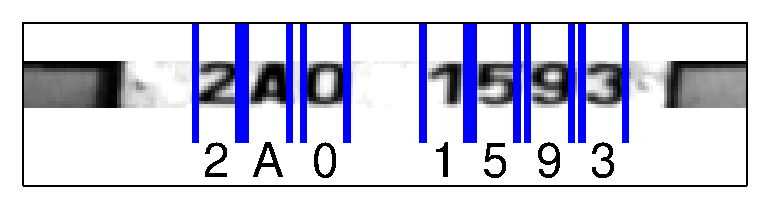
\includegraphics[width=\linewidth]{pics/input_example.eps}
\caption{Example of annotated input data. Normalized image displayed.}
\label{fig:distribution}
\end{figure}

\end{frame}

\begin{frame}
  \frametitle{Difficult data}
\begin{figure}
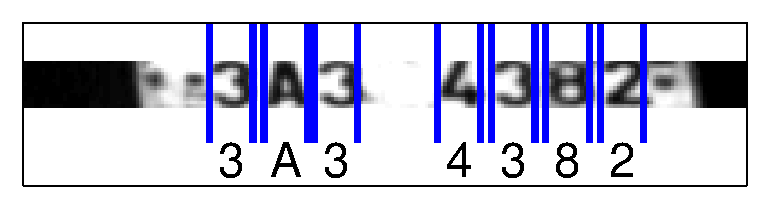
\includegraphics[width=0.8\linewidth]{pics/bad1.eps}
\end{figure}

\begin{figure}
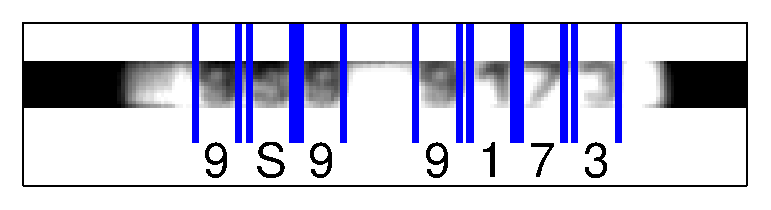
\includegraphics[width=0.8\linewidth]{pics/bad2.eps}
\end{figure}

\begin{figure}
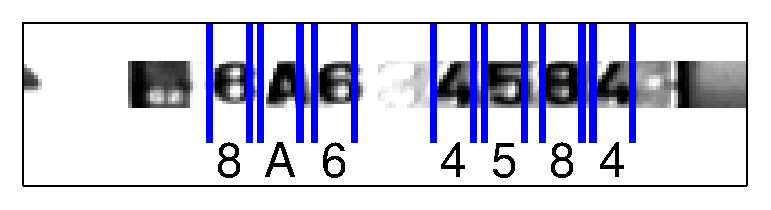
\includegraphics[width=0.8\linewidth]{pics/bad3.eps}
\end{figure}

\end{frame}


\begin{frame}
  \frametitle{Learning the emission probabilities}
	Emission probabilities of the model were learened using EM algorithm.
  
\end{frame}

\begin{frame}
  \frametitle{Learning the emission probabilities}
\begin{block}{E-step}
	\[
  p^{t+1}(x^d_{ij} \mid c=f, s_j) =
  \frac{\mathcal{N}(x^d_{ij};\sigma_1^t,\mu_1^t)\gamma_{is_j}^t}{\mathcal{N}(x^d_{ij};\sigma_1^t,\mu_1^t)\gamma_{is_j}^t+\mathcal{N}(x^d_{ij};\sigma_2^t,\mu_2^t)(1-\gamma_{is_j}^t)}
\]
	\end{block}

\begin{block}{M-step}
\[
  \gamma_{is_j}^{t+1} = \frac{\sum_{d \in \mathcal{D}} p^{t+1}(x^d_{ij} \mid
    c=f, s_j)}{\sum_{d \in \mathcal{D}} p^{t+1}(x^d_{ij} \mid c=f,
    s_j) + \sum_{d \in \mathcal{D}} (1-p^{t+1}(x^d_{ij} \mid c=b,
    s_j))}
\]
\[
  \sigma_1^{t+1} = \frac{\sum_{i,j} \sum_{d \in \mathcal{D}} x^d_{
      ij} p^{t+1}(x^d_{ij} \mid c=f, s_j)}{\sum_{i,j} \sum_{d \in
      \mathcal{D}} p^{t+1}(x^d_{ij} \mid c=f, s_j)}
\]
\end{block}  
\end{frame}

\begin{frame}
  \frametitle{Learning the emission probabilities}
\begin{itemize}
\item Stopping criterion is relative
\item  $|1-\frac{\sigma_1^{t+1}}{\sigma_1^{t}}| < \epsilon \wedge |1-\frac{\sigma_2^{t+1}}{\sigma_2^{t}}| < \epsilon$
\item$\epsilon$ has been set to value $10^{-5}$
\end{itemize}  
\end{frame}

\begin{frame}
  \frametitle{Learned templates}
\begin{figure}[htp]
\centering
\includegraphics[width=\linewidth]{pics/jba.png}
\caption{Learned templates of \texttt{J}, \texttt{B} and
  \texttt{A}. Intensity corresponds to the prior probability for being
  a foreground pixel.}
\label{fig:templates}
\end{figure}
\end{frame}




\begin{frame}
  \frametitle{Setting the transition probabilities}
  JAMES
\end{frame}


\begin{frame}
  \frametitle{Inference}
  JAMES
\end{frame}

\section{Evaluation}
\begin{frame}
  \frametitle{Evaluation}

\begin{figure}
  \centering
  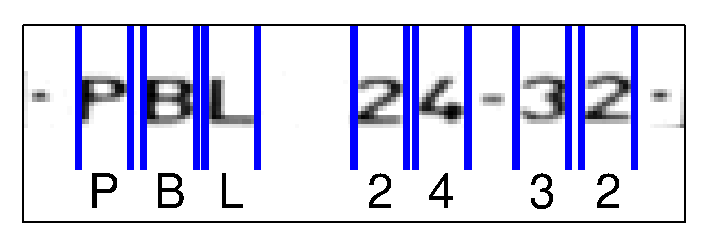
\includegraphics[width=0.6\textwidth]{pics/lic_PBL2432.eps}          
\end{figure}  
  
\begin{figure}
  \centering
  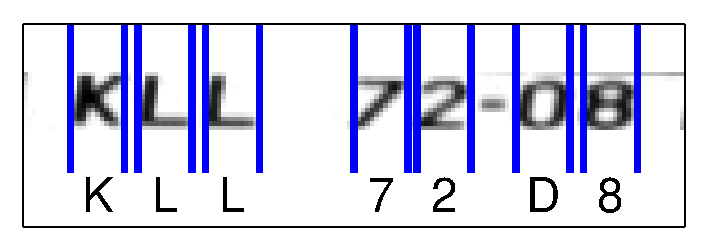
\includegraphics[width=0.6\textwidth]{pics/lic_KLL72D8.eps}
\end{figure}  

\begin{figure}
  \centering
  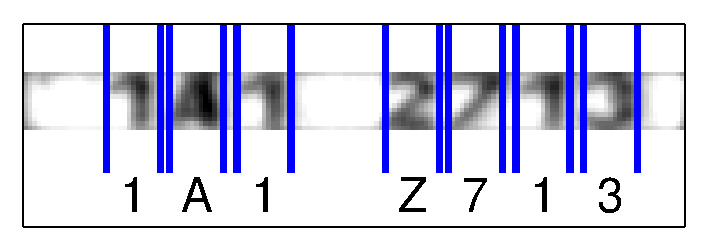
\includegraphics[width=0.6\textwidth]{pics/lic_1A1Z713.eps}
\end{figure}    
  
\end{frame}

\begin{frame}
  \frametitle{Segmentation Performance \& Accuracy}
  
  \begin{table}[ht]
\begin{center}
\begin{tabular}{|l|l|}
  \hline
  \multicolumn{2}{|c|}{Segmentation Performance} \\
  \hline
  $p_d$ & 71.9\% \\
  $p_{fa}$ & 7.60\% \\
  \hline
\end{tabular}
\caption{Calculated for \texttt{np-images-5000.mat}}
\label{table:segmentation}
\end{center}
\end{table}

\begin{table}[ht]
\begin{center}
\begin{tabular}{|l|l|}
  \hline
  \multicolumn{2}{|c|}{ID accuracy} \\
  \hline
  $accuracy$ & 36.5\% \\
  \hline
\end{tabular}
\caption{Calculated for \texttt{np-images-5000.mat}}
\end{center}
\end{table} 
  
\end{frame}

\begin{frame}
  \frametitle{Levenshtein distance}
  \begin{figure}
\begin{center}
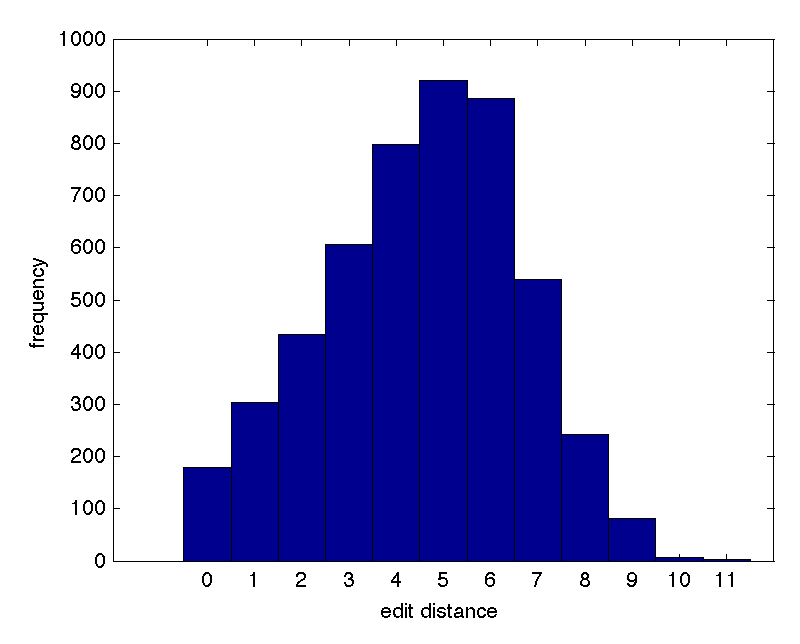
\includegraphics[width=0.75\linewidth]{pics/hamming.eps}
\caption{ Frequency of edit distance over \texttt{np-images-5000.mat}  } 
\label{fig:editdistance}
\end{center}
\end{figure}
\end{frame}

\begin{frame}
  \frametitle{Conclusions}
\end{frame}

\end{document}
